% on bueler-leopard see
%   /usr/share/doc/latex-beamer/solutions/conference-talks/conference-ornate-20min.en.tex

\documentclass{beamer}

\usetheme{Pittsburgh}
\setbeamercovered{transparent}
\setbeamertemplate{navigation symbols}{} %remove navigation symbols

\usepackage[english]{babel}
\usepackage[latin1]{inputenc}

\usepackage{times}
\usepackage[T1]{fontenc}

% see http://tex.stackexchange.com/questions/86188/labelling-with-arrows-in-an-automated-way
\usepackage{tikz}
\usepackage{amsmath}

\newif\ifclipme\clipmetrue
\tikzset{labelstyle/.style={LabelStyle/.append style={#1}},linestyle/.style={LineStyle/.append style={#1}}}
\tikzset{LabelStyle/.initial={},LineStyle/.initial={}}

\newcommand{\mathWithDescription}[4][]{{%
    \tikzset{#1}%
    \tikz[baseline]{
        \node[draw=red,rounded corners,anchor=base] (m#4) {$\displaystyle#2$};
        \ifclipme\begin{pgfinterruptboundingbox}\fi
            \node[above of=m#4,font=\strut, LabelStyle] (l#4) {#3};
            \draw[-,red, LineStyle] (l#4) to (m#4);
        \ifclipme\end{pgfinterruptboundingbox}\fi
    }%
}}

\newcommand{\mathWithDescriptionStarred}[3][]{{%
    \clipmefalse%
    \mathWithDescription[#1]{#2}{#3}{\themathLabelNode}%
}}

\newcounter{mathLabelNode}

\newcommand{\mathLabelBox}[3][]{%
   \stepcounter{mathLabelNode}%
   \mathWithDescription[#1]{#2}{#3}{\themathLabelNode}%
   \vphantom{\mathWithDescriptionStarred[#1]{#2}{#3}{\themathLabelNode}}%
}

% math macros
\newcommand\bb{\mathbf{b}}
\newcommand\bbf{\mathbf{f}}
\newcommand\bn{\mathbf{n}}
\newcommand\bq{\mathbf{q}}
\newcommand\bu{\mathbf{u}}
\newcommand\bv{\mathbf{v}}
\newcommand\by{\mathbf{y}}

\newcommand\bQ{\mathbf{Q}}
\newcommand\bV{\mathbf{V}}
\newcommand\bX{\mathbf{X}}

\newcommand\CC{\mathbb{C}}
\newcommand{\DDt}[1]{\ensuremath{\frac{d #1}{d t}}}
\newcommand{\ddt}[1]{\ensuremath{\frac{\partial #1}{\partial t}}}
\newcommand{\ddx}[1]{\ensuremath{\frac{\partial #1}{\partial x}}}
\newcommand{\ddy}[1]{\ensuremath{\frac{\partial #1}{\partial y}}}
\newcommand{\ddxp}[1]{\ensuremath{\frac{\partial #1}{\partial x'}}}
\newcommand{\ddz}[1]{\ensuremath{\frac{\partial #1}{\partial z}}}
\newcommand{\ddxx}[1]{\ensuremath{\frac{\partial^2 #1}{\partial x^2}}}
\newcommand{\ddyy}[1]{\ensuremath{\frac{\partial^2 #1}{\partial y^2}}}
\newcommand{\ddxy}[1]{\ensuremath{\frac{\partial^2 #1}{\partial x \partial y}}}
\newcommand{\ddzz}[1]{\ensuremath{\frac{\partial^2 #1}{\partial z^2}}}
\newcommand{\Div}{\nabla\cdot}
\newcommand\eps{\epsilon}
\newcommand{\grad}{\nabla}
\newcommand{\ihat}{\mathbf{i}}
\newcommand{\ip}[2]{\ensuremath{\left<#1,#2\right>}}
\newcommand{\jhat}{\mathbf{j}}
\newcommand{\khat}{\mathbf{k}}
\newcommand{\nhat}{\mathbf{n}}
\newcommand\lam{\lambda}
\newcommand\lap{\triangle}
\newcommand\Matlab{\textsc{Matlab}\xspace}
\newcommand\RR{\mathbb{R}}
\newcommand\vf{\varphi}


\title[Conservation in free-boundary layers] % (optional, use only with long paper titles)
{Conservation \\ in \\ free-boundary fluid layer \\ models}


\author{Ed Bueler}

\institute[UAF] % (optional, but mostly needed)
{
  Dept of Mathematics and Statistics, and Geophysical Institute\\
  University of Alaska Fairbanks%
}

\date{{\scriptsize AGU 2014}}


% If you have a file called "university-logo-filename.xxx", where xxx
% is a graphic format that can be processed by latex or pdflatex,
% resp., then you can add a logo as follows:
% \pgfdeclareimage[height=0.5cm]{university-logo}{university-logo-filename}
% \logo{\pgfuseimage{university-logo}}



% Delete this, if you do not want the table of contents to pop up at
% the beginning of each subsection:
%\AtBeginSection[]
%{
%  \begin{frame}<beamer>{Outline}
%    \tableofcontents[currentsection]
%    %\tableofcontents[currentsection,currentsubsection]
%  \end{frame}
%}


\begin{document}
\graphicspath{{../images/}{../../talks-public/commonfigs/}}

\begin{frame}
  \titlepage
\end{frame}

\begin{frame}{Outline}
  \tableofcontents
\end{frame}


% Structuring a talk is a difficult task and the following structure
% may not be suitable. Here are some rules that apply for this
% solution: 

% - Exactly two or three sections (other than the summary).
% - At *most* three subsections per section.
% - Talk about 30s to 2min per frame. So there should be between about
%   15 and 30 frames, all told.

% - A conference audience is likely to know very little of what you
%   are going to talk about. So *simplify*!
% - In a 20min talk, getting the main ideas across is hard
%   enough. Leave out details, even if it means being less precise than
%   you think necessary.
% - If you omit details that are vital to the proof/implementation,
%   just say so once. Everybody will be happy with that.

\section{The problem I'm worried about:}

\subsection{Free-boundary fluid layer well-posedness.}

\begin{frame}{A fluid layer in a climate}

\begin{center}
\only<1-4>{\includegraphics[width=\textwidth,keepaspectratio=true]{cartoon-layer}}
\only<5>{\includegraphics[width=\textwidth,keepaspectratio=true]{cartoon-wclimate}}
\end{center}

\vspace{-7mm}
  \begin{itemize}
  \item mass conservation for a layer:
     \only<1-4>{$$h_t + \Div\bq = f$$}
     \only<5>{$$h_t + \Div\bq = {\color{blue} f}$$}
    \begin{itemize}
    \vspace{-4mm}
    \item<2->[$\circ$] $h$ is a thickness: $h\ge 0$
    \item<3->[$\circ$] mass conservation PDE applies \emph{only where} $h>0$
    \item<4->[$\circ$] $\bq$ is flow (vertically-integrated)
    \item<5>[$\circ$] source ${\color{blue} f}$ is ``climate''; $f>0$ shown downward
    \end{itemize}
  \end{itemize}
\end{frame}


\begin{frame}{A fluid layer in a climate: \emph{the troubles}}

\begin{center}
\only<1>{\includegraphics[width=\textwidth,keepaspectratio=true]{cartoon-sensitive-three}}
\only<2>{\includegraphics[width=\textwidth,keepaspectratio=true]{cartoon-sensitive-one}}
\only<3>{\includegraphics[width=\textwidth,keepaspectratio=true]{cartoon-sensitive-two}}
\end{center}

\vspace{-18mm}
$$h_t + \Div\bq = f$$

  \begin{itemize}
  \item<1-> $h=0$ \emph{and what else} at free boundary?
     \begin{itemize}
     \item<1->[$\circ$] shape at free boundary depends on both $\bq$ and $f$
     \end{itemize}
  \item<2-> $f<0$ not ``detected'' by model where $h=0$
     \begin{itemize}
     \item<2->[$\circ$] how to do mass conservation accounting?
     \end{itemize}
  \item<3> $f\approx 0$ threshold behavior
     \begin{itemize}
     \item<3>[$\circ$] $h>0$ as soon as $f<0$ switches to $f>0$
     \end{itemize}
  \end{itemize}
\end{frame}


\begin{frame}{Examples}

\includegraphics[width=0.42\textwidth,keepaspectratio=true]{polaris}
\hfill
\includegraphics[width=0.47\textwidth,keepaspectratio=true]{supp4rignot-small}

\small glaciers \hfill ice shelves \& sea ice

\medskip
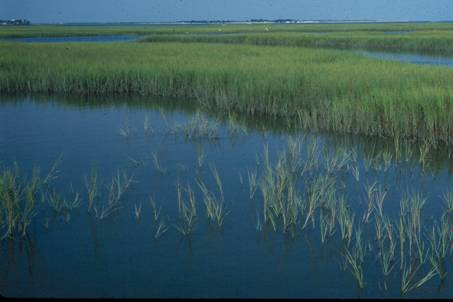
\includegraphics[width=0.43\textwidth,keepaspectratio=true]{marsh-water}
\hfill
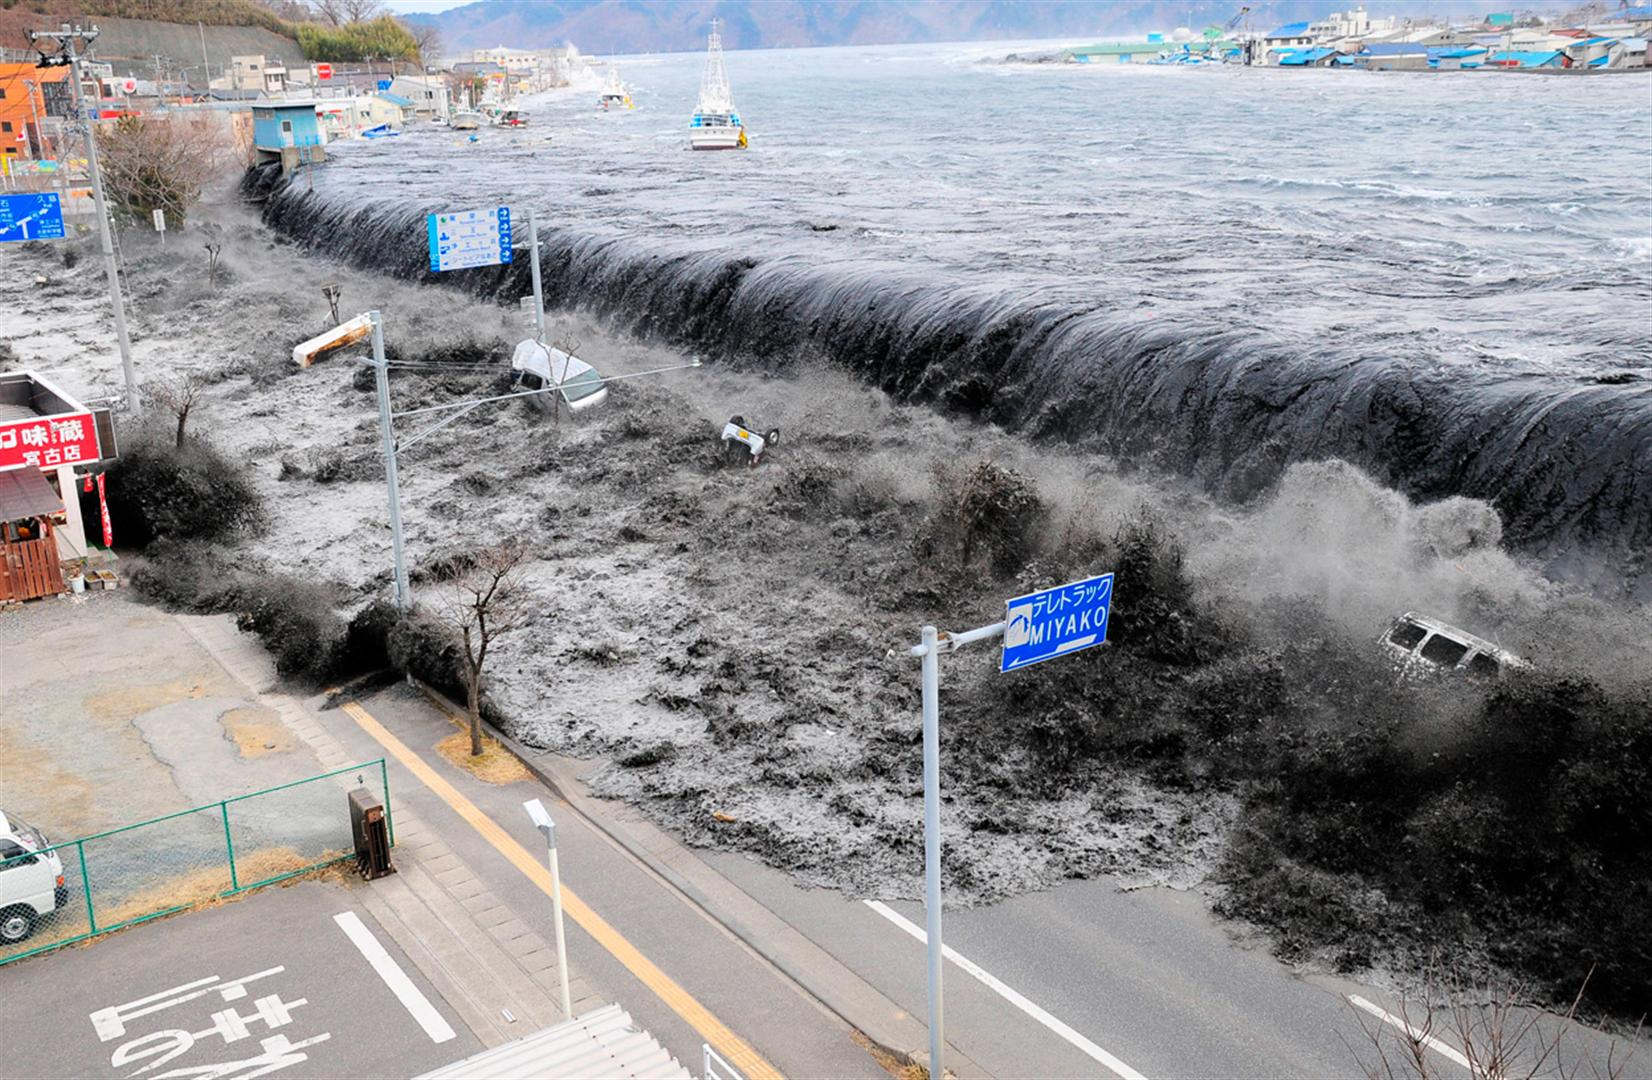
\includegraphics[width=0.44\textwidth,keepaspectratio=true]{tsunami-sendai}

\small tidewater marsh \hfill tsunami inundation

%\vspace{-2mm}
%{\tiny {\color{gray} (Alonso, Santillana \& Dawson, 2008)}}

\medskip
\scriptsize and subglacial hydrology, supraglacial runoff, surface hydrology, \dots


\end{frame}


\begin{frame}{Numerical models \emph{must} discretize time}

$$h_t + \Div\bq = f \qquad \to \qquad \frac{H_n - H_{n-1}}{\Delta t} + \Div \bQ_n = F_n$$

  \begin{itemize}
  \item semi-discretize in time: $H_n(x) \approx h(t_n,x)$
  \item<2-> new equation is ``single time-step problem''
    \begin{itemize}
    \item<2->[$\circ$] it's a PDE in space \alert{where $H_n>0$}
    \item<2->[$\circ$] I'll assume:
       \begin{itemize}
       \item<2->[$\diamond$] flux $\bQ_n$ depends on $H_n,\grad H_n,x$
       \item<2->[$\diamond$] source $F_n$ depends on $H_n,x$
       \end{itemize}
    \end{itemize}
  \item<3-> details of $\bQ_n$, $F_n$ come from time-step scheme
    \begin{itemize}
    \item<3->[$\circ$] forward/backward Euler, trapezoid, RK all o.k.
    \end{itemize}
  \item<4> low regularity of $h(t,x)$ for $x$ near margin means low accuracy expectations for time-step scheme
  \end{itemize}
\end{frame}


\begin{frame}{Anyone faced these problems before?}

  \begin{itemize}
  \item yes, of course!  for example:
    \begin{itemize}
    \item[$\circ$] ad hoc schemes for finite volume/difference mass conservation
    \end{itemize}
  \only<2>{\bigskip \item I don't mind ``\texttt{if \dots then \dots}'' in my code, \emph{but} I want to know what mathematical problem it reflects!}
  \end{itemize}

\only<1>{
\begin{columns}
\begin{column}{0.3\textwidth}
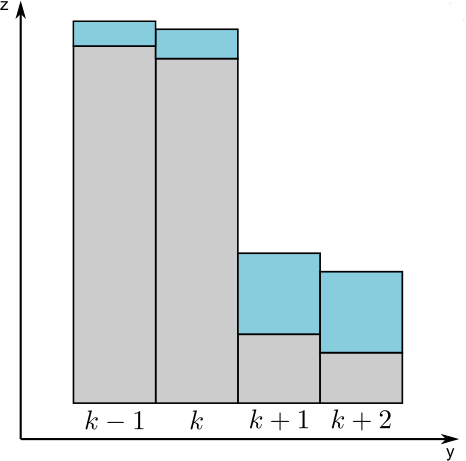
\includegraphics[width=\textwidth,keepaspectratio=true]{JaroschSchoofAnslow2013}

\small glacier ice

on steep terrain

\smallskip
\tiny (Jarosch, Schoof, Anslow, 2013)
\end{column}

\begin{column}{0.6\textwidth}
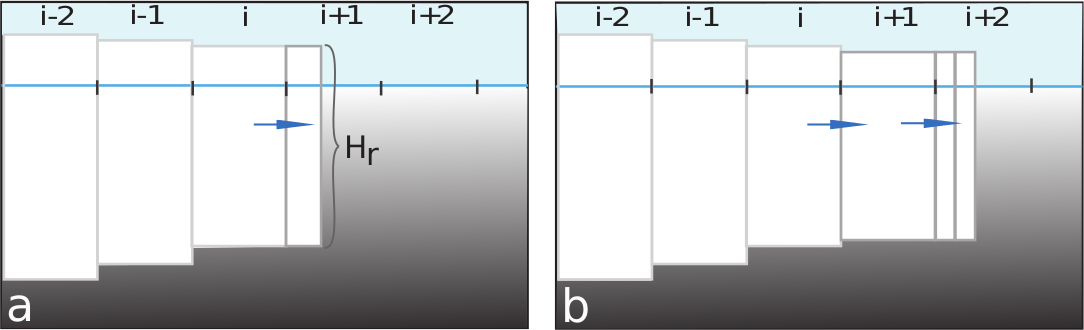
\includegraphics[width=0.8\textwidth,keepaspectratio=true]{Albrechtetal2011}

\small ice shelf fronts

\tiny (Albrecht et al, 2011)

\small \medskip
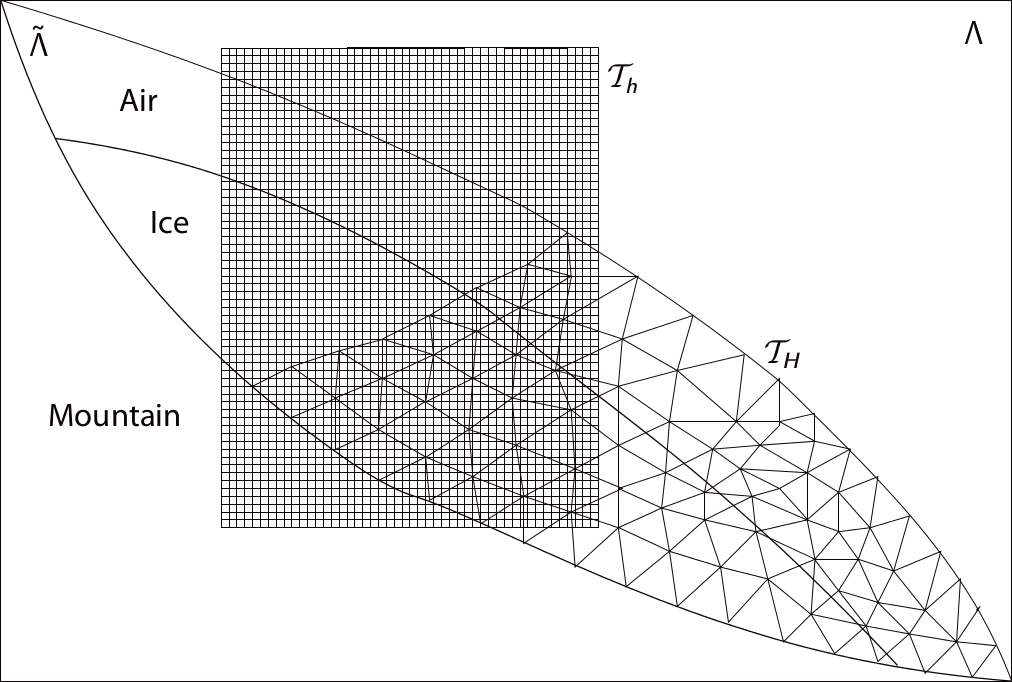
\includegraphics[width=0.6\textwidth,keepaspectratio=true]{jouvet-two-grids}

\small volume-of-fluid method on fine grid

\tiny (Jouvet et al 2008)
\end{column}
\end{columns}}

\only<2>{\phantom{foo}

\vspace{33.8mm}
\phantom{bar}}
\end{frame}


\begin{frame}{Weak form incorporates constraint}

  \begin{itemize}
  \item equation \,$\frac{H_n - H_{n-1}}{\Delta t} + \Div \bQ_n = F_n$\, is ``strong form''
  \item define set of admissible thicknesses:
    $$\mathcal{K} = \left\{v \in W^{1,p}(\Omega) \,\Big|\, v\ge 0\right\}$$
  \item<2> define: $H_n \in \mathcal{K}$ \emph{solves the weak single time-step problem} if
    $$\int_\Omega H_n (v - H_n) - \Delta t\, \bQ_n \cdot \grad(v - H_n) \ge \int_\Omega \left(H_{n-1} + \Delta t\, F_n\right) (v - H_n)$$
  for all $v \in \mathcal{K}$
  \small
  \medskip
    \begin{itemize}
    \item[$\circ$] derive this ``variational inequality'' from the strong form and integration-by-parts
    \end{itemize}
  \end{itemize}
\end{frame}


\begin{frame}{Theorem: weak solves strong}

\emph{Theorem}.  Assume $\bQ_n=0$ when $H_n=0$.  Assume $H_n \in \mathcal{K}$ solves weak single time-step problem and is smooth.  Then
  \begin{enumerate}
  \item ``interior condition'' on set where $H_n>0$:
    $$\frac{H_n - H_{n-1}}{\Delta t} + \Div \bQ_n = F_n$$
  \item on set where $H_n = 0$:
    $$H_{n-1} + \Delta t\, F_n \le 0$$
  \end{enumerate}

\uncover<2>{
re part 2:
  \begin{itemize}
  \item ``climate is negative enough to remove old thickness''
  \item it is nontrivial: assumption ``$\bQ_n=0$ when $H_n=0$'' is needed
    \begin{itemize}
    \item[$\circ$] \dots yes, we are talking about a \emph{layer}
    \end{itemize}
  \end{itemize}}
\end{frame}


\section{Practical consequences:}

\subsection{Limits to auditable discrete conservation.}

\begin{frame}{Sets for single time-step problem}
\begin{itemize}
\item $\Omega$ is the (fixed) computational domain
\item suppose $H_n$ solves the weak single time-step problem
\item define
	\begin{align*}
	\Omega_n &= \left\{x \in \Omega\,\Big|\,H_n(x) > 0\right\} \\
	\Omega_n^r &= \left\{x \in \Omega\,\Big|\,H_n(x)= 0 \text{ and } H_{n-1}(x) > 0\right\} \quad \text{\alert{retreat set}}
	\end{align*}
\end{itemize}

\vspace{-2mm}
\begin{center}
\includegraphics[width=1.0\textwidth,keepaspectratio=true]{cartoon-sets}
\end{center}
\end{frame}


\begin{frame}{Discrete mass conservation}

\begin{itemize}
\item define:
   $$M_n = \int_\Omega H_n(x)\,dx \qquad \text{\emph{mass at time} $t_n$}$$
\item then \vspace{-5mm}
	\begin{align*}
	M_n - M_{n-1} &= \int_{\Omega_n} \mathLabelBox[
    labelstyle={xshift=2cm},
    linestyle={out=270,in=90, -latex}
    ]{H_n - H_{n-1}}{$\boxed{\Delta t\, (-\Div\bQ_n + F_n)}$} \,dx + \int_{\Omega_n^r} 0 - H_{n-1} \,dx \\
	   &= \Delta t\, \left(0 + \int_{\Omega_n} F_n \,dx\right) - \int_{\Omega_n^r} H_{n-1} \,dx
	\end{align*}
\item change in mass is from
  \begin{itemize}
  \item[$\circ$] climate over fluid-covered region: $C_n = \Delta t\, \int_{\Omega_n} F_n \,dx$
  \item[$\circ$] another term:
     $$R_n = \int_{\Omega_n^r} H_{n-1} \,dx \qquad \text{\emph{\alert{retreat loss} during step} $n$}$$
  \end{itemize}
\end{itemize}
\end{frame}


\begin{frame}{Discrete conservation: \emph{main claim}}

\begin{itemize}
\item \alert{the retreat loss $R_n$ is not balanced by the climate}
  \begin{itemize}
  \item[$\circ$] yes, $R_n$ \emph{is} ``caused'' by the climate, but we don't know what computable integral it balances
  \end{itemize}

\medskip
\item thus a numerical model must track \alert{three} time series to ``balance the books'':
  \begin{itemize}
  \item[$\circ$] mass at time $t_n$: $M_n = \int_\Omega H_n(x)\,dx$
  \item[$\circ$] climate over fluid-covered region:
     $$C_n = \Delta t\, \int_{\Omega_n} F_n \,dx = \int_{t_{n-1}}^{t_n} \int_{\Omega_n} F_n \,dx\,dt$$
  \item[$\circ$] retreat loss: $R_n = \int_{\Omega_n^r} H_{n-1} \,dx$
  \end{itemize}
\item so that
  $$M_n = M_{n-1} + C_n - R_n$$
\end{itemize}
\end{frame}


\subsection{Numerical variational inequality solution needed.}

\begin{frame}{FIXME}
\end{frame}


\section*{Summary}

\begin{frame}{Summary}

  % Keep the summary *very short*.
  \begin{itemize}
  \item
    The \alert{first main message} of your talk in one or two lines.
  \item
    The \alert{second main message} of your talk in one or two lines.
  \item
    Perhaps a \alert{third message}, but not more than that.
  \end{itemize}
  
  % The following outlook is optional.
  \vskip0pt plus.5fill
  \begin{itemize}
  \item
    Outlook
    \begin{itemize}
    \item
      Something you haven't solved.
    \item
      Something else you haven't solved.
    \end{itemize}
  \end{itemize}
\end{frame}


\end{document}


